\documentclass[a4paper,12pt]{report}

\usepackage{xcolor}
\usepackage{float}
\usepackage{comment}
\usepackage{graphicx}
\usepackage[utf8]{inputenc}
\usepackage[italian]{babel}
\usepackage{array}
\usepackage[hidelinks]{hyperref}
\usepackage{verbatim}

\title{Report per progetto di basi di dati\\ MixologyDB\\ \small Gruppo num.\normalsize 2999\\ \large A.A. 2025/2026\\}

\author{
    \textbf{\vspace{0.1cm}Valente Domenico} \\
     0001171156 \\
    \texttt{domenico.valente4@studio.unibo.it}
}

\date{\today}
\begin{document}

\maketitle

\tableofcontents
\newpage

\section{Analisi dei requisiti}
\begin{flushleft}
Si vuole progettare un database su cui creare un'applicazione desktop per visualizzare, salvare e condividere ricette, preparazioni e ingredienti per cocktail esistenti e riconosiuti dalla rivista IBA o creati dagli utenti.
\end{flushleft}

\subsection{Intervista}
L'obiettivo principale è la progettazione e lo sviluppo di un database a supporto di un'applicazione desktop pensata per gli appassionati di mixology. La piattaforma si presenta come un raccoglitore digitale in cui, inizialmente, il sistema metterà a disposizione un catalogo preimpostato, contenente i cocktail più celebri, ufficialmente riconosciuti dall'IBA (International Bartenders Association), aggiornati fino ad una certa data, ma sarà possibile inserire nuove creazioni.\\
\\
La \textbf{parte centrale} dell'applicativo è la seguente:\\
Ogni drink, che sia un classico IBA o una nuova creazione, sarà descritto in maniera precisa e comprenderà informazioni importanti sulla sua composizione. Il sistema terrà traccia non solo del nome e dell'eventuale utente creatore, ma anche della categoria di appartenenza e di una descrizione generale.\\
In pratica, verranno memorizzati gli ingredienti necessari compresi di foto e keywords per facilitarne l'individuazione e la categorizzazione.\\
Gli utenti si interfacceranno con il sistema tramite due livelli di accesso:\\
gli \textbf{utenti  non registrati} potranno esplorare il catalogo senza interagirvi: non potranno creare ricette, scrivere recensioni ...\\
Al contrario, un \textbf{utente registrato} diventerà parte attiva della community: potrà arricchire il database creando e pubblicando nuovi drink personalizzati. Inoltre, sarà possibile salvare i drink nella sezione \textit{"preferiti"}, aggiungere recensioni testuali alle ricette ed esportare (salvando su file) i dati di un drink, per poter condividere la ricetta.\\
Il sistema prevede la registrazione di \textbf{bar}. Ogni bar è associato ad un certo numero di \textit{utenti registrati}, da cui possono aggiungere una creazione "di gruppo".
\\
Per navigare nell'archivio, l'applicazione fornirà un motore di ricerca in cui gli utenti potranno cercare un drink non solo per nome, ma anche filtrando per gusti (ad esempio "dolce", "amaro", "fruttato"), per specifici ingredienti (come "gin" o "fragola"), o sfruttando le parole chiave inserite liberamente dai creatori.\\
\\
\\
Alcuni utenti specifici saranno dotati dei privilegi di \textit{"Amministratore"}. Il loro compito principale sarà quello di mantenere l'ambiente pertinente e rispettoso. Gli amministratori avranno quindi il potere di intervenire eliminando ricette inappropriate o recensioni non pertinenti e potranno rimuovere definitivamente gli account degli utenti che violano le linee guida. Ogni amministratore avrà accesso a una lista completa degli iscritti, arricchita da dati statistici che aiutino a identificare anomalie, in modo da facilitare la moderazione della piattaforma.\\
\\
Infine, il database dovrà supportare la possibilità di ottenere di informazioni aggregate, generando statistiche e tendenze in un dato periodo. Il sistema sarà in grado di calcolare e mostrare le classifiche degli ingredienti più utilizzati dalla community e dei gusti di maggiore tendenza in un dato periodo. Sarà inoltre possibile premiare l'impegno degli utenti evidenziando coloro che ricevono il maggior numero di recensioni positive.


\subsection{Estrazione dei concetti principali}

\begin{tabular}{|l|p{8cm}|}
\hline
\textbf{Utente registrato}\normalsize: &persona che può interagire con il database, visualizzando e aggiungendo determinate informazioni;\\
\hline
\textbf{Bar}: &"gruppo" di barman che possono interagire con il database visualizzando le informazioni \footnotesize(proprio come gli \textit{utenti})\normalsize e registrando informazioni in gruppo;\\
\hline
\textbf{Admin}: &utente dotato di permessi "speciali" che si occupa della moderazione;\\
\hline
\textbf{Drink}: &Componente fondamentale, contiene le informazioni minime che identificano e descrivono un qualsiasi drink;\\
\hline
\textbf{Ingrediente}: &Componente aggiuntivo, contiene informazioni riguardandti la composizione del drink;\\
\hline
\textbf{Categoria}: &Componente aggiuntivo, permette di categorizzare correttamente i drink;\\
\hline
\textbf{Tag}: &componente aggiuntivo, associa ad un drink un certo numero di keyword. Svolgono un ruolo fondamentale per la ricerca dei drink all'interno del database.\\
\hline
\end{tabular}

\subsection{Correzione delle ambiguità}
\subsubsection{Segue un testo che riassume i concetti più a basso livello, eliminandone le ambiguità:}

Per ogni utente registrato vengono salvati nome, cognome, e-mail e password e, dopo la prima iscrizione, potrà autenticarsi accedendo con la sua e-mail e password. Un utente registrato può visualizzare i drink già presenti nel database e crearne di nuovi, anche tramite il suo bar.\\
un utente non registrato, al contrario, non sarà abilitato fruire delle seguenti funzioni: creare drink, scrivere recensioni, salvare drink come \textit{"preferiti"}.\\
Tutti gli utenti saranno abilitati alla \textit{ricerca tramite parole chiave}, utilizzando le parole chiave che il creatore del drink ha specificato, oltre la descrizione stessa del drink. 
Vi sarà la possibilità, solo per utenti specifici, di accedere come "admin", per moderare l'uso della piattaforma. 

\subsubsection{Più specificatamente, per un utente registrato, il programma offrirà le seguenti funzionalità:}
\begin{enumerate}
    \item salvataggio di drink nella scheda personale “preferiti”;
    \item Salvataggio su file pdf dei dati dei drink;
    \item Ricerca di un drink tramite parole chiave.
\end{enumerate}

\subsubsection{Invece, l'amministratore sarà abilitato ad eseguire le seguenti operazioni:}
\begin{enumerate}
    \item Eliminare ricette non pertinenti;
    \item Eliminare recensioni non pertinenti;
    \item Eliminare gli autori di ricette e/o recensioni non pertinenti;
    \item Ottenere una lista di tutti gli utenti, compresa di alcune informazioni aggregate, per facilitare il processo di moderazione.
\end{enumerate}

\subsubsection{Inoltre, sarà possibile visualizzare le seguenti informazioni aggregate:}
\begin{enumerate}
    \item Elenco degli utenti con più recensioni positive;
    \item Elenco degli ingredienti più utilizzati;
    \item Elenco degli elementi di tendenza;
    \item Raccomandazione di drink in base ai drink preferiti dell’utente;
    \item Il drink con più recensioni positive in un determinato periodo di tempo (ad esempio il più recensito del mese).
\end{enumerate}

\subsection{elenco delle principali azioni richieste}
\begin{enumerate}
    \item Iscrizione di un nuovo utente;
    \item Aggiunta di un nuovo bar, compreso di utenti dipendenti;
    \item Aggiungere una nuova creazione, categorizzarla, aggiungere parole chiave e specificarne gli ingredienti;
    \item Salvare un drink come "preferito";
    \item Ottenere la lista dei drink "preferiti";
    \item Recensire un drink;
    \item Ricerca di drink tramite nome del drink, parole chiave o descrizione;
    \item Calcolare una classifica dei $n$ drink con recensioni migliori nel periodo recente;
    \item Visualizzare l'elenco degli ingredienti più utilizzati;
    \item Calcolare una classifica dei $n$ utenti che hanno ottenuto più recensioni positive;
    \item Visualizzare la lista dei gusti di tendenza;

    
    \item Suggerimento di drink ad un utente, in base al contenuto dei suoi preferiti;   
    \item (per gli amministratori) ottenere una lista degli utenti iscritti, comprensiva di dati analitici utili per la moderazione;
    \item (per gli amministratori) Eliminazione di una recensione o di una ricetta segnalata come inopportuna;    
    \item (per gli amministratori) Eliminazione di un utente dal sistema per violazione delle linee guida, con cancellazione a cascata di recensioni e lista "preferiti", mantenimento delle ricette come anonime.
\end{enumerate}


\newpage
\section{Progettazione Concettuale}


\subsection{Schema scheletro}

\subsubsection{Gestione degli utenti}
La modellazione di questo aspetto risulta particolarmente semplice:
\\
l'entità \textit{Utente registrato} modella un utente che può interagire attivamente col database ed essere aggiunto tra i dipendenti di un bar. Ad ogni \textit{Utente registrato} viene attribuito un codice identificativo (non viene usata l'email per non escludere la possibilità di poterla cambiare in futuro).
\\\\
\textit{numeroDipendenti} è un attributo ridondante: bisognerà valutarne l’utilità durante la fase di progettazione logica.

\begin{figure}[H]
    \centering
    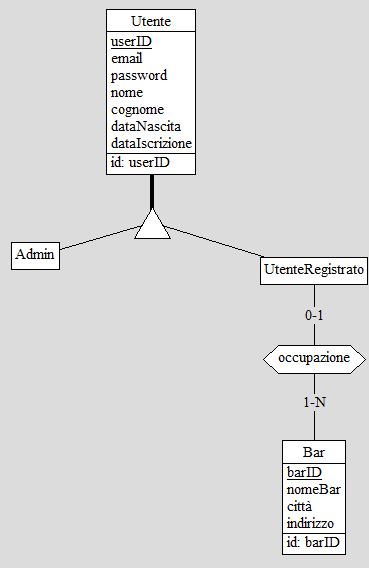
\includegraphics[width=0.5\linewidth]{images/concettuale/scheletro1.png}
    \caption{Schema ER contenente le principali entità e relazioni per la modellazione degli utenti e dei bar}
    \label{ER_scheletro_utenti}
\end{figure}


\subsubsection{Gestione delle ricette (Drink)}

L'entità \textit{Drink} si riferisce ad una generica ricetta con una descrizione e un'immagine. Vengono attribute una \textit{categoria} (con annessa descrizione), una o più \textit{keywords} per facilitarne la ricerca e uno o più ingredienti (specificando quantità e unità di misura).
\begin{itemize}
    \item \textit{IBA} è un booleano: indica se quel drink è tra quelli già presenti nel database dall'inizio.
    \item \textit{numeroIngredienti} è un attributo ridondante, bisognerà valutarne l'utilità durante la fase di progettazione logica.
\end{itemize}
\begin{figure}[H]
    \centering
    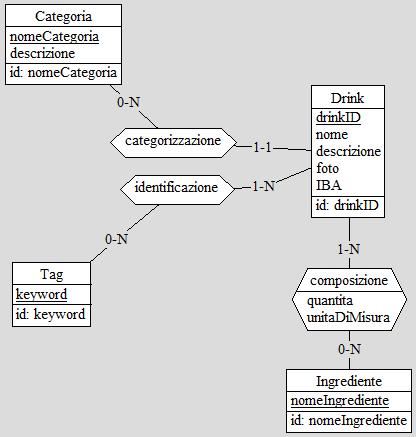
\includegraphics[width=0.8\linewidth]{images/concettuale/scheletro2.png}
    \caption{Schema ER contenente le principali entità e relazioni per la modellazione delle diverse ricette e la loro composizione, categorizzazione e identificazione}
    \label{ER_scheletro_drink}
\end{figure}

\subsubsection{gestione delle relazioni Utente-Drink}
Tutti gli utenti registrati e amministratori possono condividere ricette, salvare ricette come "preferite" e recensirle.

\begin{itemize}
    \item Ogni \textit{Utente} potrà creare e recensire fino a $n$ drink, ma dovrà poter lasciare una sola recensione per drink.\\
    \textbf{Soluzione}: \textit{salvataggio preferiti} e \textit{recensisce} sono relazioni, impedendo ad un utente di salvare o recensire più volte la stessa ricetta.
    \item \textit{numeroRicetteCreate}, \textit{numeroRecensioniEffettuate}, \textit{numeroDipendenti}, \textit{numeroPreferitiSalvati} sono attributi ridondanti: bisognerà valutarne l'utilità durante la fase di progettazione logica.
\end{itemize}
\begin{figure}[H]
    \centering
    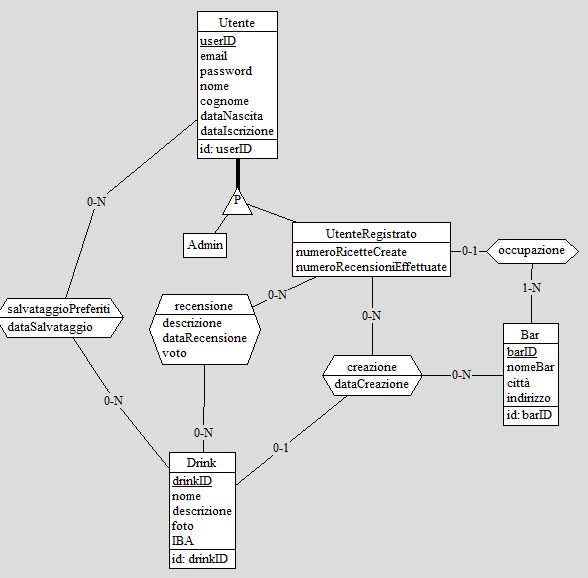
\includegraphics[width=0.95\linewidth]{images/concettuale/scheletro3.png}
    \caption{Schema ER raffigurante le principali operazioni che gli utenti possono fare sulle ricette}
    \label{ER_scheletro_user-drink}
\end{figure}

\subsection{Schema concettuale completo}

\begin{figure}[H]
    \centering
    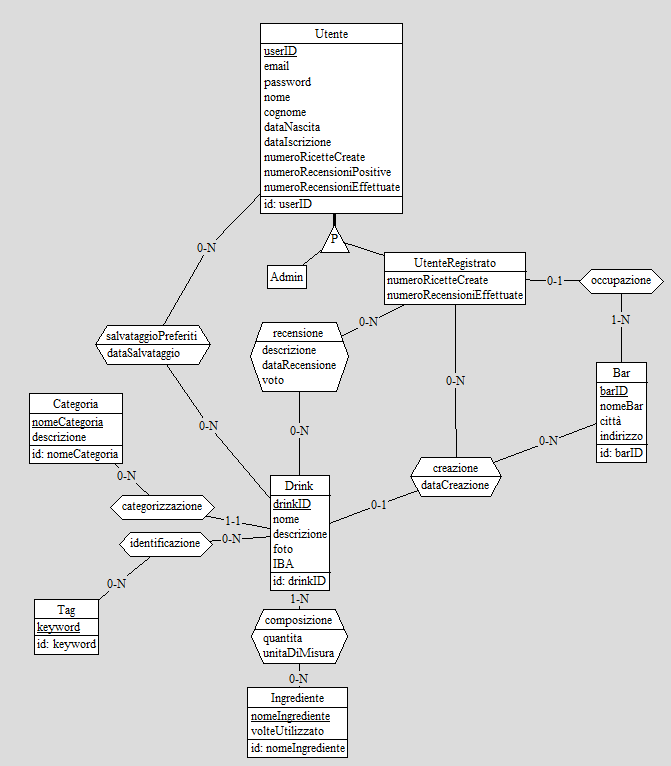
\includegraphics[width=1.1\linewidth]{images/concettuale/concettualeCompleto.png}
    \caption{Schema ER completo}
    \label{fig:placeholder}
\end{figure}

\newpage
\section{Progettazione logica}
\subsection{Stima dei volumi}

\renewcommand{\arraystretch}{1.3} 
\begin{tabular}{c|c|c}
    concetto & costrutto & volume\\
\hline
    \small UtenteRegistrato\normalsize & E & 10.000\\
    \hline
    Admin & E & 5 $^*$ \\
    \hline
    Bar & E & 200\\
    \hline
    occupazione & R & 600\\
\hline
\end{tabular}
\\
\\
\\
\renewcommand{\arraystretch}{1.3} 
\begin{tabular}{c|c|c}
    concetto & costrutto & volume\\
\hline
    Drink & E & 20.100\tiny(circa 100 IBA)\normalsize\\
    \hline
    creazione & R & 15.000\\
    \hline
    recensione & R & 60.000\\
    \hline
    \footnotesize salvataggioPreferiti\normalsize & R & 300.000\\
\hline
\end{tabular}
\\
\\
\\
\renewcommand{\arraystretch}{1.3} 
\begin{tabular}{c|c|c}
    concetto & costrutto & volume\\
\hline
    Categoria & E & 20\\
    \hline
    categorizzazione & R & 20.100\\
    \hline
    Tag & E & 1.500\\
    \hline
    identificazione & R & 60.300\\
    \hline
    ingrediente & E & 500\\
    \hline
    composizione & R & 110.500\tiny(media di 5 per ogni drink)\\
\hline
\end{tabular}

\footnote{$^*$: Il conteggio è stato effettuato considerando UtenteRegistrato+Admin=10.005. Spiegazione durante la fase di raffinamento: \ref{raffinamentoSchema}}

\newpage
\subsection{Operazioni principali e stima della loro frequenza}

\renewcommand{\arraystretch}{1.7} %%%%%%%%%%%% 
\begin{tabular}{c|c|c} 
    codice & operazione & frequenza\\
\hline
\hline
    1 & Iscrizione di un nuovo utente & 50/w\\
    \hline
    2 & Aggiunta di un nuovo bar & 3/w\\
    \hline
    3 & Aggiungere una nuova creazione & 400/w\\
    \hline
    4 & salvare un drink come preferito & 10.000/w\\
    \hline
    5 & ottenere la lista dei preferiti & 4.000/w\\
    \hline 
    6 & recensire un drink & 1.200/w\\
    \hline
    7 & Ricerca di drink tramite nome keyword o descrizione & 80.000/w\\
    \hline
    8 & visualizzare la classifica dei drink attualmente meglio recensiti & 10.000/w\\
    \hline
    9 & Elenco degli ingredienti più utilizzati & 8.000/w\\
    \hline
    10 & utenti con più recensioni positive & 8.000/w\\
    \hline
    11 & lista dei gusti di tendenza & 40.000/w\\
    \hline
    12 & Suggerimento di drink ad un utente in base ai suoi salvati & 40.000/w\\
    \hline
    13 & \small(admin)\normalsize ottenere una lista di utenti compresa di dati analitici & 20/w\\
    \hline
    14 & \small(admin)\normalsize eliminazione di recensioni o ricette inopportune & 100/w\\
    \hline
    15 & \small(admin)\normalsize ban di un utente & 10/w\\    
\hline
\end{tabular}

\newpage
\subsection{Raffinamento dello schema}
\label{raffinamentoSchema}
\subsubsection{Eliminazione delle gerarchie}
Per l'eliminazione della gerarchia su "Utente" si è deciso di applicare un collasso verso l'alto, dato il numero di attributi e la relazione in comune. Per distinguere amministratori e utenti, si è deciso di aggiungere un attributo "ruoloUtente" (Admin/User), in modo tale da distinguere i due ruoli.

\subsubsection{Eliminazione degli attributi composti}
Lo schema non presenta attributi composti: i concetti che potrebbero richiederlo sono già stati modellati tramite attributi.
\\
\subsubsection{Scelta delle chiavi primarie}
Si è scelto di attribuire un codice univoco agli utenti, per non escludere a priori la possibilità di poter cambiare la mail in futuro.
\\
Per quanto riguarda l'entità "Tag", "Categoria" e "Ingrediente", si è scelto di utilizzare i rispettivi nominativi, essendo univoci. Questa scelta, inoltre, aumenta l'efficienza durante l'inserimento di dati.

\begin{figure}[H]
    \centering
    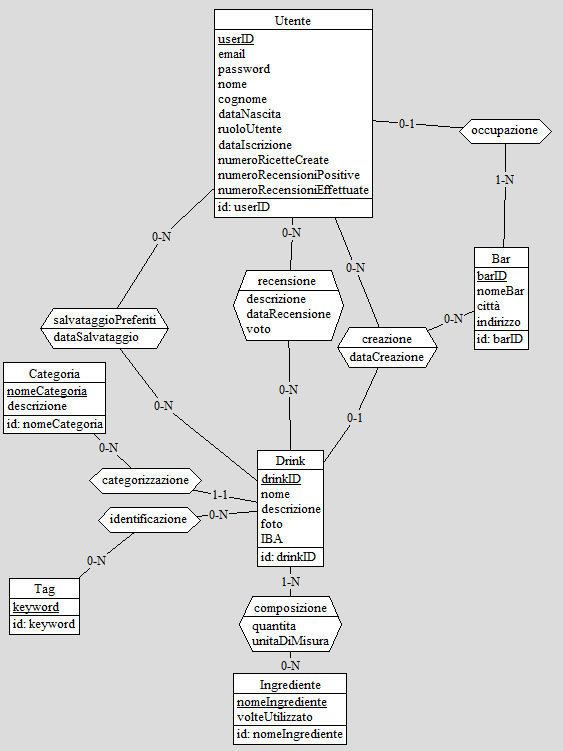
\includegraphics[width=0.95\linewidth]{images/concettuale/rivisitato.png}
    \caption{Schema ER rivisitato, è stato effettutato il collasso verso l'alto sull'entità "Utente".}
    \label{ER_rivisitato}
\end{figure}

\newpage
\subsection{Tabelle degli accessi e analisi delle ridondanze}
\renewcommand{\arraystretch}{1.4} %%%%%%%%%%%% 

\subsubsection{Analisi senza ridondanza}
\begin{enumerate}
    \item Iscrizione di un nuovo utente\\
    \begin{tabular}{c|c|c}
    concetto & accessi & tipo\\
    \hline
        Utente & 1 & S\\
    \hline
    \end{tabular}
    \\1S $\to$ 2 operazioni.

    \item Aggiunta di un nuovo Bar\\
    \begin{tabular}{c|c|c}
    concetto & accessi & tipo\\
    \hline
        Bar & 1 & S\\
        occupazione & 3 & S\\
    \hline
    \end{tabular}
    \\4S $\to$ 8 operazioni.

    \item Aggiunta di una nuova creazione \footnotesize da parte di un utente\\ \normalsize
    \begin{tabular}{c|c|c}
    concetto & accessi & tipo\\
    \hline
        Drink & 1 & S\\
        categorizzazione & 1 & S\\
        identificazione & 3 & S\\
        composizione & 5 & S\\
        creazione & 1 & S\\
    \hline
    \end{tabular}
    \\11S $\to$ 22 operazioni.

    \item Salvataggio di un drink come "preferito"\\
    \begin{tabular}{c|c|c}
    concetto & accessi & tipo\\
    \hline
        SalvataggioPreferiti & 1 & S\\
    \hline
    \end{tabular}
    \\1S $\to$ 2 operazioni.

    \item Ottenere la lista dei drink ”preferiti”\\
    \begin{tabular}{c|c|c}
    concetto & accessi & tipo\\
    \hline
        SalvataggioPreferiti & \textasciitilde 30 & L\\
        Drink & ~30 & L\\
    \hline
    \end{tabular}
    \\60L $\to$ 60 operazioni.
\footnote{\textasciitilde $30=29.98$: il calcolo è stato effettuato con un volume da 10.005 utenti: \\5 Admin e 10.000 utenti registrati.}

    \item recensire un drink\\
    \begin{tabular}{c|c|c}
    concetto & accessi & tipo\\
    \hline
        recensione & 1 & S\\
    \hline
    \end{tabular}
    \\ $1S\to2$ operazioni.

    \item Ricerca tramite parole chiave\\
    \begin{tabular}{c|c|c}
    concetto & accessi & tipo\\
    \hline
        Drink & 20.100 & L\\
        identificazione & 60.300 & L\\
        composizione & 100.500 & L\\
    \hline
    \end{tabular}
    \\ $180.900L\to180.900$ operazioni.

    \item classifica dei $n$ drink con recensioni migliori\\
        \begin{tabular}{c|c|c}
    concetto & accessi & tipo\\
    \hline
        recensione & 60.000 & L\\
    \hline
    \end{tabular}
    \\ $60.010L\to60.010$ operazioni.

    \item elenco degli ingredienti più utilizzati\\
    \begin{tabular}{c|c|c}
    concetto & accessi & tipo\\
    \hline
        composizione & 110.500 & L\\
    \hline
    \end{tabular}
    \\ $110.500L\to110.500$ operazioni.

    \item Classifica degli utenti con più recensioni positive\\
    \begin{tabular}{c|c|c}
    concetto & accessi & tipo\\
    \hline
        recensione & 60.000 & L\\
        creazione & 15.000 & L\\
        Utente & 10 & L\\
    \hline
    \end{tabular}
    \\ $75.010L\to75.010$ operazioni.

    \item Gusti di tendenza\\
    \begin{tabular}{c|c|c}
    concetto & accessi & tipo\\
    \hline
        identificazione & 60.300 & L\\
        recensione & 60.000 & L\\
    \hline
    \end{tabular}
    \\ $120.300L\to120.300$ operazioni.

    \item Suggerimenti basati sul contenuto dei "preferiti"\\
    \begin{tabular}{c|c|c}
    concetto & accessi & tipo\\
    \hline
        salvataggioPreferiti & ~30 & L\\
        categorizzazione & 30 & L\\
        identificazione & 90 & L\\
        composizione & 150 L\\
        Drink & 30 & L\\
    \hline
    \end{tabular}
    \\ $330L\to330$ operazioni.

    \item \normalsize(admin) lista di utenti e dati analitici \footnotesize (numero di recensioni, numero di ricette create e data di iscrizione)\normalsize\\
    \begin{tabular}{c|c|c}
    concetto & accessi & tipo\\
    \hline
        Utente & 10.000 & L\\
        creazione & 15.000 & L\\
        recensione & 60.000 & L\\
    \hline
    \end{tabular}
    \\ $85.000L\to85.000$ operazioni.

    \item (admin) eliminazione di ricette o recensioni non opportune\\
    \begin{tabular}{c|c|c}
    concetto & accessi & tipo\\
    \hline
        recensione & 3 & S\\
        drink & 1 & S\\
        categorizzazione & 1 & S\\
        identificazione & 3 & S\\
        composizione & 5 & S\\
        salvataggioPreferiti & 15 & S\\
    \hline
    \end{tabular}
    \\ $28S\to56$ operazioni.

    \item (admin) ban di un utente, con cancellazione di recensioni e "preferiti" e mantenimento delle ricette\\
        \begin{tabular}{c|c|c}
    concetto & accessi & tipo\\
    \hline
        Utente & 1 & S\\
        creazione & 1.5 & S\\
        recensione & 6 & S\\
        salvataggioPreferiti & 30 & S\\
    \hline
    \end{tabular}
    \\ $37.5S\to77$ operazioni.
\end{enumerate}

\begin{center}
\setlength{\tabcolsep}{18pt} % Aumenta lo spazio orizzontale (regola questo numero)
\renewcommand{\arraystretch}{1.5} % Opzionale: aumenta anche l'altezza se vuoi
\begin{tabular}{c|c|c|c}
op & accessi & frequenza/sett & totale \\
\hline
\hline
1 & 2 & 50 & 100 \\ \hline
2 & 8 & 3 & 24 \\ \hline
3 & 22 & 400 & 8.800 \\ \hline
4 & 2 & 10.000 & 20.000 \\ \hline
5 & 60 & 4.000 & 240.000 \\ \hline
6 & 2 & 1.200 & 2.400 \\ \hline
7 & 180.900 & 80.000 & 14.472.000.000 \\ \hline
8 & 60.010 & 10.000 & 600.100.000 \\ \hline
9 & 110.500 & 8.000 & 884.000.000 \\ \hline
10 & 75.010 & 8.000 & 600.080.000 \\ \hline
11 & 120.300 & 40.000 & 4.812.000.000 \\ \hline
12 & 330 & 40.000 & 13.200.000 \\ \hline
13 & 85.000 & 20 & 1.700.000 \\ \hline 
14 & 56 & 100 & 5.600 \\ \hline
15 & 77 & 10 & 770 \\ \hline \hline
\multicolumn{3}{r|}{TOTALE:} & 21.383.357.694 acc/sett \\
\end{tabular}
\end{center}

\newpage
\subsubsection{Analisi con ridondanza}
\begin{enumerate}
    \item Iscrizione di un nuovo utente\\
    \begin{tabular}{c|c|c}
    concetto & accessi & tipo\\
    \hline
        Utente & 1 & S\\
    \hline
    \end{tabular}
    \\1S $\to$ 2 operazioni.

    \item Aggiunta di un nuovo Bar\\
    \begin{tabular}{c|c|c}
    concetto & accessi & tipo\\
    \hline
        Bar & 1 & S\\
        occupazione & 3 & S\\
    \hline
    \end{tabular}
    \\4S $\to$ 8 operazioni.

    \item Aggiunta di una nuova creazione \footnotesize da parte di un utente\\ \normalsize
    \begin{tabular}{c|c|c}
    concetto & accessi & tipo\\
    \hline
        Utente & 1 & A\\
        Drink & 1 & S\\
        categorizzazione & 1 & S\\
        identificazione & 3 & S\\
        composizione & 5 & S\\
        creazione & 1 & S\\
    \hline
    \end{tabular}
    \\12S + 1L $\to$ 25 operazioni.

    \item Salvataggio di un drink come "preferito"\\
    \begin{tabular}{c|c|c}
    concetto & accessi & tipo\\
    \hline
        SalvataggioPreferiti & 1 & S\\
    \hline
    \end{tabular}
    \\1S $\to$ 2 operazioni.

    \item Ottenere la lista dei drink ”preferiti”\\
    \begin{tabular}{c|c|c}
    concetto & accessi & tipo\\
    \hline
        SalvataggioPreferiti & \textasciitilde 30 & L\\
        Drink & ~30 & L\\
    \hline
    \end{tabular}
    \\60L $\to$ 60 operazioni.
\footnote{\textasciitilde $30=29.98$: il calcolo è stato effettuato con un volume da 10.005 utenti: \\5 Admin e 10.000 utenti registrati.}

    \item recensire un drink\\
    \begin{tabular}{c|c|c}
    concetto & accessi & tipo\\
    \hline
        recensione & 1 & S\\
        Utente & 2 & A\\
    \hline
    \end{tabular}
    \\ $3S + 2L\to 8$ operazioni.

    \item Ricerca tramite parole chiave\\
    \begin{tabular}{c|c|c}
    concetto & accessi & tipo\\
    \hline
        Drink & 20.100 & L\\
        identificazione & 60.300 & L\\
        composizione & 100.500 & L\\
    \hline
    \end{tabular}
    \\ $180.900L\to180.900$ operazioni.

    \item classifica dei $n$ drink con recensioni migliori\\
        \begin{tabular}{c|c|c}
    concetto & accessi & tipo\\
    \hline
        recensione & 60.000 & L\\
        Drink & 10 & L\\
    \hline
    \end{tabular}
    \\ $60.010L\to60.010$ operazioni.

    \item elenco degli ingredienti più utilizzati\\
    \begin{tabular}{c|c|c}
    concetto & accessi & tipo\\
    \hline
        ingrediente & 500 & L\\
    \hline
    \end{tabular}
    \\ $500L\to500$ operazioni.

    \item Classifica degli utenti con più recensioni positive\\
    \begin{tabular}{c|c|c}
    concetto & accessi & tipo\\
    \hline
        Utente & 10.005 & L\\
    \hline
    \end{tabular}
    \\ $ 10.005L\to 10.005$ operazioni.

    \item Gusti di tendenza\\
    \begin{tabular}{c|c|c}
    concetto & accessi & tipo\\
    \hline
        identificazione & 60.300 & L\\
        recensione & 60.000 & L\\
    \hline
    \end{tabular}
    \\ $120.300L\to120.300$ operazioni.

    \item Suggerimenti basati sul contenuto dei "preferiti"\\
    \begin{tabular}{c|c|c}
    concetto & accessi & tipo\\
    \hline
        salvataggioPreferiti & ~30 & L\\
        categorizzazione & 30 & L\\
        identificazione & 90 & L\\
        composizione & 150 L\\
        Drink & 30 & L\\
    \hline
    \end{tabular}
    \\ $330L\to330$ operazioni.

    \item \normalsize(admin) lista di utenti e dati analitici \footnotesize (numero di recensioni, numero di ricette create e data di iscrizione)\normalsize\\
    \begin{tabular}{c|c|c}
    concetto & accessi & tipo\\
    \hline
        Utente & 10.005 & L\\
    \hline
    \end{tabular}
    \\ $10.005L\to10.005$ operazioni.

    \item (admin) eliminazione di ricette non opportune\\
    \begin{tabular}{c|c|c}
    concetto & accessi & tipo\\
    \hline
        recensione & 3 & S\\
        drink & 1 & S\\
        categorizzazione & 1 & S\\
        identificazione & 3 & S\\
        composizione & 5 & S\\
        salvataggioPreferiti & 15 & S\\
        Utente  & 15 & A\\
        Ingrediente (agg. contatori) & 5 & A\\

    \hline
    \end{tabular}
    \\ $27S + 21A \to 117$ operazioni.

    \newpage
    \item (admin) ban di un utente, con cancellazione di recensioni e "preferiti" e mantenimento delle ricette\\
        \begin{tabular}{c|c|c}
    concetto & accessi & tipo\\
    \hline
        Utente & 1 & S\\
        Utente & 6 & A\\
        creazione & 1.5 & S\\
        recensione & 6 & S\\
        salvataggioPreferiti & 30 & S\\
    \hline
    \end{tabular}
    \\ $37S + 7.5A \to 96.5$ operazioni.
\end{enumerate}

\begin{center}
\setlength{\tabcolsep}{18pt} % Aumenta lo spazio orizzontale (regola questo numero)
\renewcommand{\arraystretch}{1.5} % Opzionale: aumenta anche l'altezza se vuoi
\begin{tabular}{c|c|c|c}
op & accessi & frequenza/sett & totale \\
\hline
\hline
1 & 2 & 50 & 100 \\ \hline
2 & 8 & 3 & 24 \\ \hline
3 & 25 & 400 & 10.000 \\ \hline
4 & 2 & 10.000 & 20.000 \\ \hline
5 & 60 & 4.000 & 240.000 \\ \hline
6 & 8 & 1.200 & 9.600 \\ \hline
7 & 180.900 & 80.000 & 14.472.000.000 \\ \hline
8 & 60.010 & 10.000 & 600.100.000 \\ \hline
9 & 500 & 8.000 & 4.000.000 \\ \hline
10 & 10.005 & 8.000 & 80.040.000 \\ \hline
11 & 120.300 & 40.000 & 4.812.000.000 \\ \hline
12 & 330 & 40.000 & 13.200.000 \\ \hline
13 & 10.005 & 20 & 200.100 \\ \hline 
14 & 117 & 100 & 11.700 \\ \hline
15 & 96.5 & 10 & 965 \\ \hline \hline
\multicolumn{3}{r|}{TOTALE:} & 19.981.831.289 acc/sett \\
\end{tabular}
\end{center}

\newpage
\subsubsection{Conclusione}
\normalsize La variante con ridondanza risulta essere nettamente più efficiente, specialmente nelle operazioni 8 e 9, le quali, nella variante senza ridodnanza, richiederebbero la lettura di un volume intero.
\\
Per questo motivo, verrà usata la versione con ridondanza.

\subsection{Traduzione di entità e associazioni in relazioni}
\large
\textbf{Utenti} (\underline{userID}, email, password, nome, cognome, dataNascita, ruoloUtente, dataIscrizione, numeroRicetteCreate, numeroRecensioniPositive, numeroRecensioniEffettuate)\\
\textbf{occupazioni} (Utenti: \underline{userID}, Bar: \underline{barID})\\
\textbf{Bar} (\underline{barID}, nomeBar, città, indirizzo)\\
\textbf{creazioni} (Utenti: \underline{userID}, Drink: \underline{drinkID}, barID*,  dataCreazione)\\
\textbf{recensioni}: (Utenti: \underline{userID}, Drink: \underline{drinkID}, descrizione, dataRecensione, voto)\\
\textbf{salvataggioPreferiti}: (Utenti: \underline{userID}, Drink: \underline{drinkID}, dataSalvataggio)\\
\textbf{Drink} (\underline{drinkID}, nomeCategoria, nome, descrizione, foto, nomeCategoria, IBA)\\
\textbf{Categoria} (\underline{nomeCategoria}, descrizione)\\
\textbf{Tag}: (\underline{keyword})\\
\textbf{identificazione} (Drink: \underline{drinkID}, Tag: \underline{keyword})\\
\textbf{ingredienti}: (\underline{nomeIngrediente}, volteUtilizzato)\\
\textbf{composizione: } (Drink: \underline{drinkID}, Ingredienti: \underline{nomeIngrediente}, quantita, unitaDiMisura)
\normalsize
\subsection{Schema relazionale}
\begin{figure}[H]
    \centering
    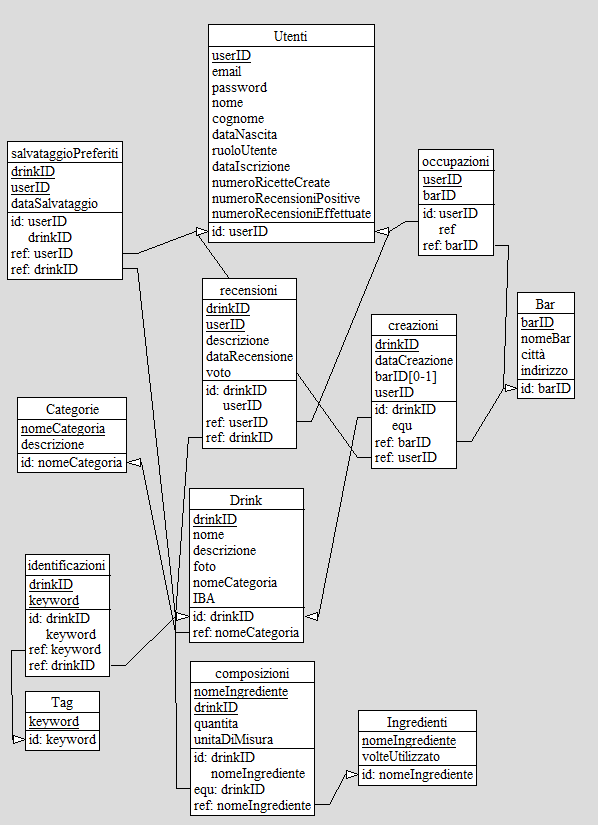
\includegraphics[width=0.9\linewidth]{images/logico/relazionaleCompleto.png}
    \caption{Schema relazionale completo}
    \label{fig:logicoCompleto}
\end{figure}
\newpage
\section{Traduzione delle operazioni in query SQL}

\subsection{File ddl}
\scriptsize
\begin{flushleft}
\verbatiminput{MixologyDB.ddl}
\end{flushleft}
\normalsize

\newpage
\subsection{Query SQL}

    Gli identificatori Drink.drinkID, User.userID, Bar.barID sono di tipo tipo int auto\textunderscore increment, pertanto non è necessario inserirli manualmente.
\begin{enumerate}
    \item \textbf{Iscrizione di un nuovo utente:}\\
        \textcolor{blue}{INSERT INTO} Utenti \footnotesize(email, password, nome, cognome, dataNascita, ruoloUtente, dataIscrizione, numeroRicetteCreate, numeroRecensioniPositive, numeroRecensioniEffettuate) \normalsize \\
        \textcolor{blue}{VALUES} (?, ?, ?, ?, ?, ?, \textcolor{gray}{DATE(NOW())}, 0, 0, 0);
        \\\\
        E per effettuare l'accesso:\\
        \textcolor{blue}{SELECT} *\\
        \textcolor{blue}{FROM} Utenti\\
        \textcolor{blue}{WHERE} email = ?\\
        \textcolor{blue}{AND} password = ?;
        
    \item \textbf{Aggiunta di un nuovo bar con dipendenti:\\}
        \textcolor{blue}{INSERT INTO} Bar (nomeBar, città, indirizzo) \\
        \textcolor{blue}{VALUES} (?, ?, ?);
        \\\\
        E per inserire i dipendendi:\\
        \textcolor{blue}{INSERT INTO} occupazioni (userID, barID)\\
        \textcolor{blue}{VALUES} (?, ?);
    
    \item \textbf{Aggiungere una nuova creazione, categorizzarla, aggiungere parole chiave e specificarne gli ingredienti (da un utente):\\}
        -- Inserimento del Drink\\
        \textcolor{blue}{INSERT INTO} Drink \footnotesize(nome, descrizione, foto, nomeCategoria, IBA)\normalsize\\
        \textcolor{blue}{VALUES} (?, ?, ?, ?, false);
        \\\\
        -- Collegamento con l'utente creatore\\
        \textcolor{blue}{INSERT INTO} creazioni (drinkID, dataCreazione, userID)\\
        \textcolor{blue}{VALUES} (?, \textcolor{gray}{DATE(NOW())}, ?);
        \\\\
        -- Inserimento ingredienti (da ripetere per ogni ingrediente)\\
        \textcolor{blue}{INSERT INTO} composizioni (nomeIngrediente, drinkID, quantita, unitaDiMisura)\\
        \textcolor{blue}{VALUES} (?, ?, ?, ?);
        \\\\
        -- Aggiornamento contatore dell'ingrediente (da ripetere per ogni ingrediente)\\
        \textcolor{blue}{UPDATE} Ingredienti\\
        \textcolor{blue}{SET} volteUtilizzato = volteUtilizzato+1\\
        \textcolor{blue}{WHERE} nomeIngrediente = ?;
        \\\\
        -- Inserimento dei Tag (da ripetere per ogni keyword)\\
        \textcolor{blue}{INSERT INTO} identificazioni (drinkID, keyword)\\
        \textcolor{blue}{VALUES} (?, ?);
        \\\\
        -- Aggiornamento del contatore creazioni dell'Utente\\
        \textcolor{blue}{UPDATE} Utenti\\
        \textcolor{blue}{SET} numeroRicetteCreate = numeroRicetteCreate+1\\
        \textcolor{blue}{WHERE} userID = ?;
        \\\\
        Il processo di categorizzazione, identificazione,... di un drink sarà gestito tramite \textbf{transazioni}. 
    
    \item \textbf{Salvare un drink come "preferito":\\}
        \textcolor{blue}{INSERT INTO} salvataggioPreferiti (drinkID, userID, dataSalvataggio)\\
        \textcolor{blue}{VALUES} (?, ?, \textcolor{gray}{DATE(NOW())});
    
    \item \textbf{Ottenere la lista dei drink "preferiti":\\}
        \textcolor{blue}{SELECT} D.*\\
        \textcolor{blue}{FROM} Utenti U, salvataggioPreferiti SP, Drink D\\
        \textcolor{blue}{WHERE} U.userID = SP.userID\\
        \textcolor{blue}{AND} SP.drinkID = D.drinkID\\
        \textcolor{blue}{AND} U.userID = ?;
        
    \item \textbf{Recensire un drink:\\}
        \textcolor{blue}{INSERT INTO} recensioni \footnotesize(drinkID, userID, descrizione, dataRecensione, voto)\\ \normalsize
        \textcolor{blue}{VALUES} (?, ?, ?, \textcolor{gray}{DATE(NOW())}, ?);
        \\\\
        Aggiorna l'attributo ridondante dell'utente che ha scritto la recensione:\\
        \textcolor{blue}{UPDATE} utenti\\
        \textcolor{blue}{SET} numeroRecensioniEffettuate = numeroRecensioniEffettuate+1\\
        \textcolor{blue}{WHERE} userID = ?;
        \\\\
        Per aggiornare l'attributo "numeroRecensioniPositive" del proprietario della ricetta, La seguente query verrà eseguita dopo una verifica sul voto della recensione:\\
        if voto $>$ 2:\\
            \textcolor{blue}{UPDATE} utenti\\
            \textcolor{blue}{SET} numeroRecensioniPositive = numeroRecensioniPositive+1\\
            \textcolor{blue}{WHERE} userID = ?;
        \\\\
        Le recensioni di un drink saranno gestite  tramite \textbf{transazioni}. 

            
    \item \textbf{Ricerca di drink tramite nome del drink, parole chiave o descrizione:}\\
    \textcolor{blue}{SELECT DISTINCT} D.*\\
    \textcolor{blue}{FROM} Drink D\\
    \textcolor{blue}{LEFT JOIN} identificazioni I \\
    \textcolor{blue}{ON} D.drinkID = I.drinkID\\
    \textcolor{blue}{LEFT JOIN} composizioni C \\
    \textcolor{blue}{ON} D.drinkID = C.drinkID\\
    \textcolor{blue}{WHERE} D.nome = ?\\
    \textcolor{blue}{OR} I.keyword = ?\\
    \textcolor{blue}{OR} C.nomeIngrediente = ?\\
    \textcolor{blue}{OR} D.nomeCategoria = ?\\
    \textcolor{blue}{OR} D.descrizione \textcolor{gray}{LIKE CONCAT('\%', ?, '\%')};
    \\\\
    Viene usato il LEFT JOIN per escludere la possibilità che, non trovando la corrispondenza con uno degli attributi, escluda a priori il drink.
            
        \item \textbf{Calcolare una classifica dei $n$ drink con più recensioni positive nel periodo recente}\\       
        \textcolor{blue}{SELECT} D.*, \textcolor{blue}{COUNT}(*) \textcolor{blue}{AS} numero\\
        \textcolor{blue}{FROM} Drink D, recensioni R\\
        \textcolor{blue}{WHERE} D.drinkID = R.drinkID\\
        \textcolor{blue}{AND} voto $>$ 2\\
        \textcolor{blue}{AND} \textcolor{gray}{DATEDIFF}(\textcolor{gray}{NOW()}, R.dataRecensione) $<=$ ?\\
        \textcolor{blue}{GROUP by} D.drinkId, D.nome, D.foto\\
        \textcolor{blue}{ORDER BY} \textcolor{blue}{COUNT}(R.voto) \textcolor{blue}{DESC}\\
        \textcolor{blue}{LIMIT} ?;
            
    \item \textbf{Visualizzare l’elenco degli ingredienti più utilizzati}\\ 
        \textcolor{blue}{SELECT} *\\
        \textcolor{blue}{FROM} ingredienti\\
        \textcolor{blue}{ORDER BY} volteUtilizzato \textcolor{blue}{DESC}\\
        \textcolor{blue}{LIMIT} ?;
    
    \item \textbf{Visualizzare la classifica degli utenti che hanno ottenuto più recensioni positive}\\
        \textcolor{blue}{SELECT} *\\
        \textcolor{blue}{FROM} utenti\\
        \textcolor{blue}{ORDER BY} numeroRecensioniPositive \textcolor{blue}{DESC}\\
        \textcolor{blue}{LIMIT} ?;
        
    \item \textbf{ Visualizzare la lista dei gusti di tendenza}\\
        \textcolor{blue}{SELECT} keyword, \textcolor{blue}{COUNT}(*) \textcolor{blue}{AS} tendenza\\
        \textcolor{blue}{FROM} identificazioni I, recensioni R\\
        \textcolor{blue}{WHERE} I.drinkID = R.drinkID\\
        \textcolor{blue}{AND} \textcolor{blue}{DATEDIFF}(\textcolor{gray}{DATE(NOW())}, R.dataRecensione) $<=$ ?\\
        \textcolor{blue}{AND} R.voto $>$ 2\\
        \textcolor{blue}{GROUP BY} keyword\\
        \textcolor{blue}{ORDER BY} tendenza \textcolor{blue}{DESC}
        \textcolor{blue}{LIMIT} ?;
        \\\\
    
    \item \textbf{Suggerimento di drink ad un utente, in base al contenuto dei suoi salvati}\\
        \textcolor{blue}{SELECT DISTINCT} D.*\\
        \textcolor{blue}{FROM} Drink D, identificazioni I\\
        \textcolor{blue}{WHERE} D.drinkID = I.drinkID\\
        \textcolor{blue}{AND} I.keyword \textcolor{blue}{IN}\\
        (\textcolor{blue}{SELECT} I2.keyword\\
        \textcolor{blue}{ FROM} salvataggioPreferiti SP, identificazioni I2\\
        \textcolor{blue}{WHERE} I2.drinkID = SP.drinkID\\
        \textcolor{blue}{AND} SP.userID = ?)\\
        \textcolor{blue}{AND} D.drinkID \textcolor{blue}{NOT IN}\\
        (\textcolor{blue}{SELECT} drinkID \\
        \textcolor{blue}{FROM} salvataggioPreferiti SP2\\
        \textcolor{blue}{WHERE} SP2.userID = ?)\\
        \textcolor{blue}{LIMIT} ?;
        \\\\
        Il suggerimento deve essere basato sulle keywords associate ai propri drink preferiti, ma ovviamente i drink usati per la ricerca non devono comparire nei suggerimenti.\\
        Soluzione: escludo i drink salvati dall'utente (NOT IN ...)
        
    \item \textbf{\textcolor{orange}{Admin} | ottenere una lista degli utenti iscritti, comprensiva di dati analitici utili per la moderazione}\footnotesize (numero di recensioni, numero di ricette create e data di iscrizione)\normalsize\\
    \textcolor{blue}{SELECT} *\\
    \textcolor{blue}{FROM} utenti;\\
    \\
    E per vedere le recensioni che ha fatto:\\
    \textcolor{blue}{SELECT} R.*\\
    \textcolor{blue}{FROM} utenti U, recensioni R\\
    \textcolor{blue}{WHERE} U.userID = R.userID\\
    \textcolor{blue}{AND} U.userID = ?;
    
    \item \textbf{\textcolor{orange}{Admin} | Eliminazione di una recensione o di una ricetta inopportuna}\\
    Per eliminare una recensione:\\
        \textcolor{blue}{DELETE FROM} recensioni\\
        \textcolor{blue}{WHERE} drinkId = ?\\
        \textcolor{blue}{AND} userID = ?;\\

    Per eliminare una ricetta:\\
        \textcolor{blue}{DELETE FROM} drink\\
        \textcolor{blue}{WHERE} drinkID = ?;
        \\\\
        Avendo specificato "ON DELETE CASCADE", il database, al momento dell'eliminazione di una recensione o di una ricetta, elimina automaticamente le relazioni ad esso associate.
    
    \item \textbf{\textcolor{orange}{Admin} | ban di un utente dal sistema con cancellazione a cascata di recensioni e lista "preferiti", mantenimento delle ricette come anonime}\\
        Soluzione: Verrà inserito nel database un utente anonimo con userID = 0, a cui verranno associate le ricette appartenenti agli utenti eliminati.
        \\
        prima di tutto, vengono assegnate le creazioni appartenenti all'utente da eliminare all'utente anonimo, per non perderle.\\
        \textcolor{blue}{UPDATE} creazioni\\
        \textcolor{blue}{SET} userID = 1\\
        \textcolor{blue}{WHERE} userID = ?;\\
        \\
        Una volta segnate le ricette come anonime, elimina l'utente.\\
        \textcolor{blue}{DELETE FROM} utenti\\
        \textcolor{blue}{WHERE} userID = ?;
        
\end{enumerate}


\newpage
\section{Progettazione dell'applicazione}
\subsection{Descrizione dell’applicazione}
L’applicazione per interfacciarsi al database è stata realizzata in Java, usando la libreria JDBC; il database risiede in locale e il DBMS usato è mySQL.\\
L’applicazione è un semplice programma in swing, la quale usa una DatabaseConnection per interfacciarsi con il dataBase e creare interfacce DAO.
\\
Si è cercato di ridurre i controlli non necessariamente da svolgere a livello applicativo facendo verifiche a livello del DBMS.

\subsubsection{Registrazione/Login}
Una volta avviato il programma, vi sarà la possibilità di effettuare il login, registrarsi o entrare come ospite.

\begin{figure}[H]
    \centering
    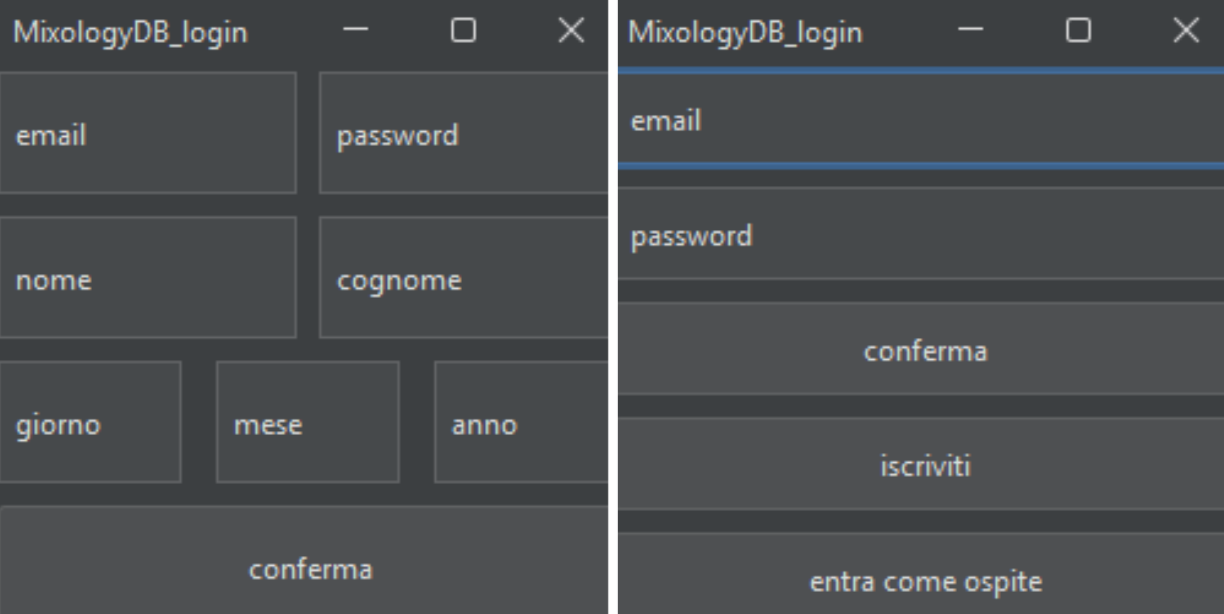
\includegraphics[width=0.9\linewidth]{images/applicazione/loginForm.png}
    \caption{form di login/registrazione}
    \label{fig:loginForm}
\end{figure}

\newpage
\subsubsection{schermata principale}
Ovviamente, come visibile nelle figure \ref{fig:mainPanel} e \ref{fig:guestMainPanel}, nel caso un utente decidesse di entrare come ospite, non sarà abilitato a svolgere operazioni di scrittura sul database.
\\

\begin{figure}[H]
    \centering
    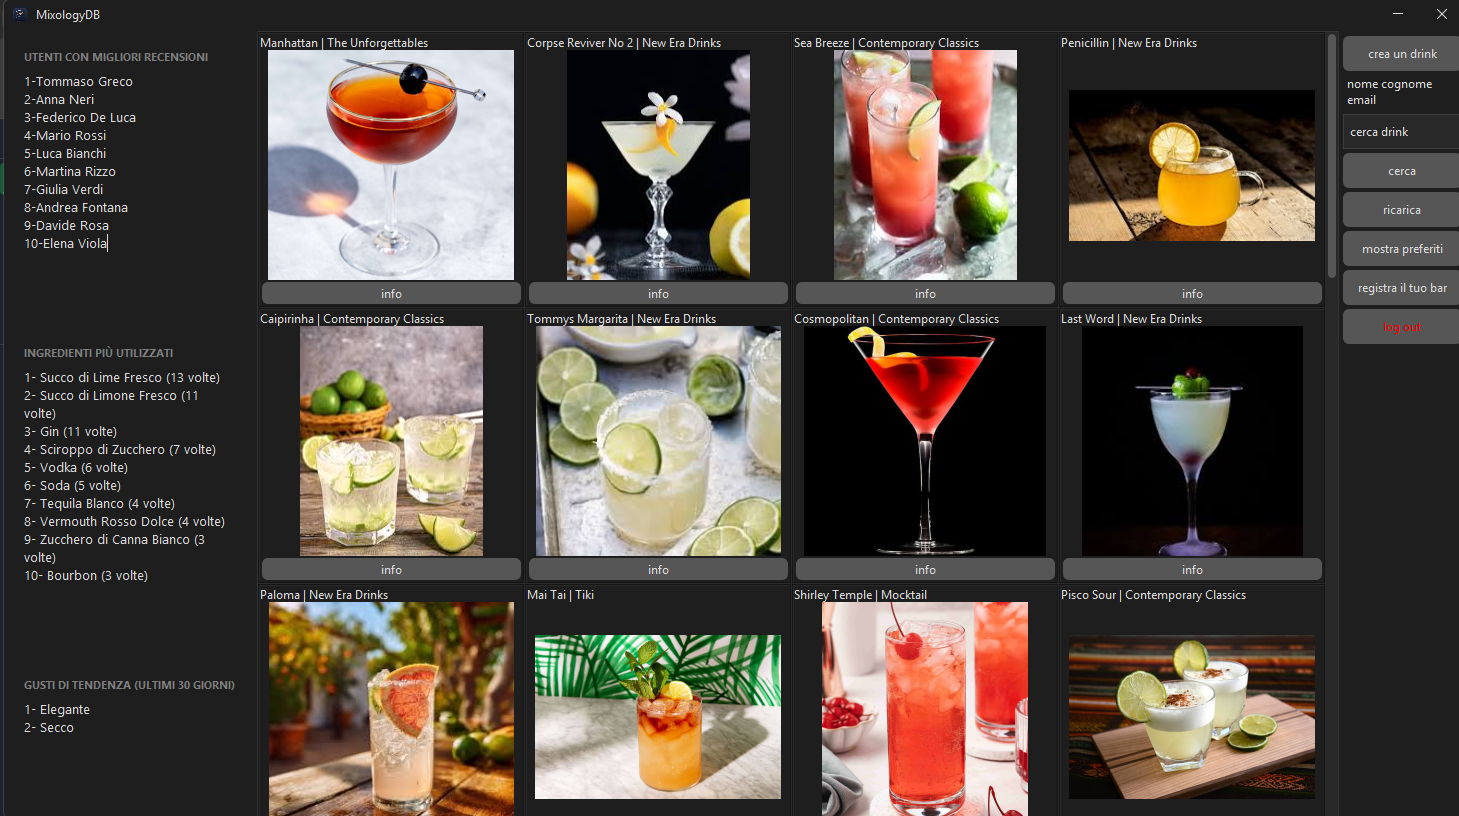
\includegraphics[width=0.8\linewidth]{images/applicazione/schermataPrincipale.png}
    \caption{schermata principale per gli utenti registrati}
    \label{fig:mainPanel}
\end{figure}

\begin{figure}[H]
    \centering
    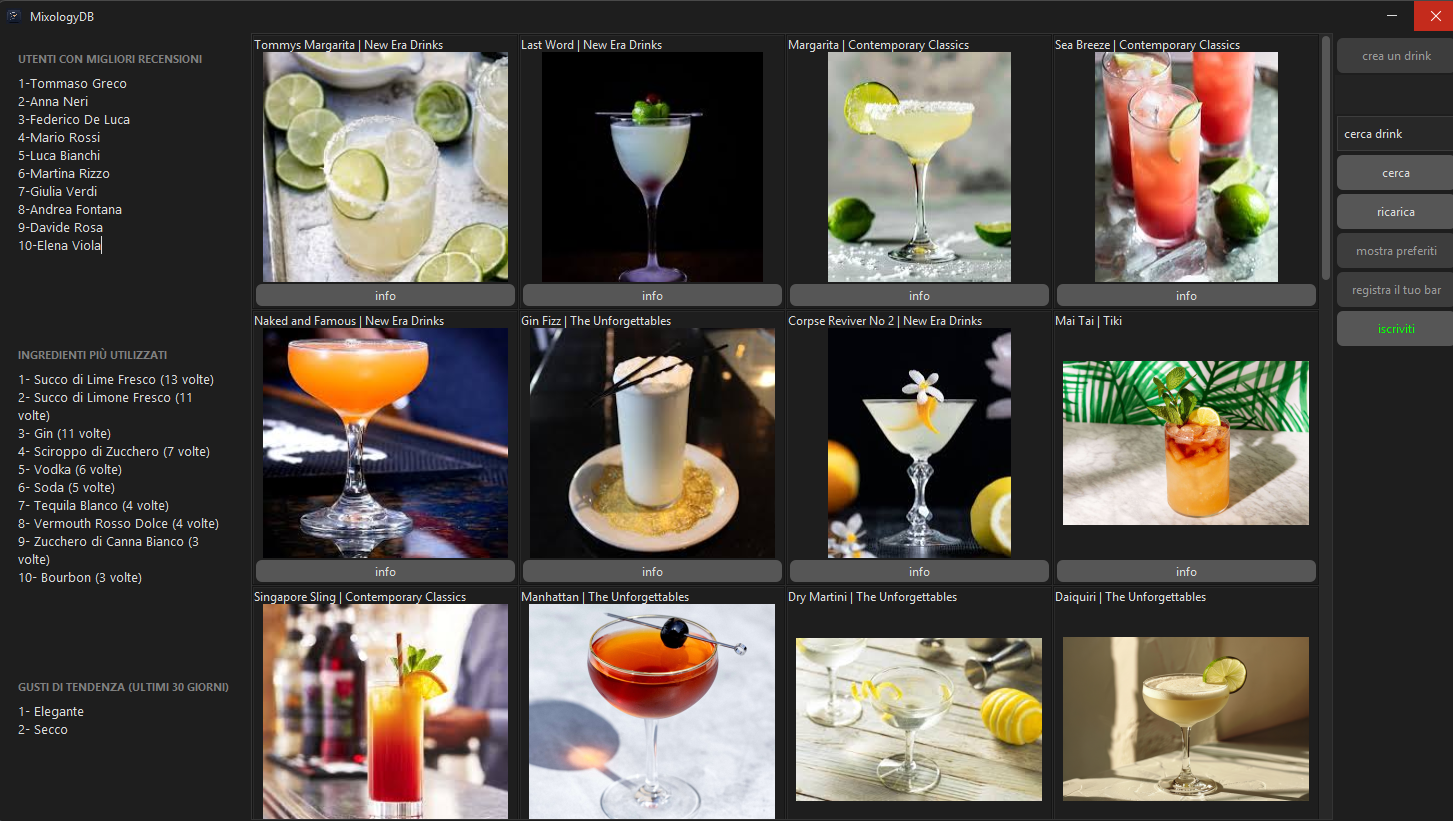
\includegraphics[width=0.8\linewidth]{images/applicazione/guest1.png}
    \caption{schermata principale per gli ospiti}
    \label{fig:guestMainPanel}
\end{figure}

\newpage
\subsubsection{Ricerca per parole chiave}
E' possibile cercare ricette tramite parole chiave. nella figura \ref{fig:keyWordSearch} viene cercato l'ingrediente "rum" *\ref{*1}. 

\begin{figure}[H]
    \centering
    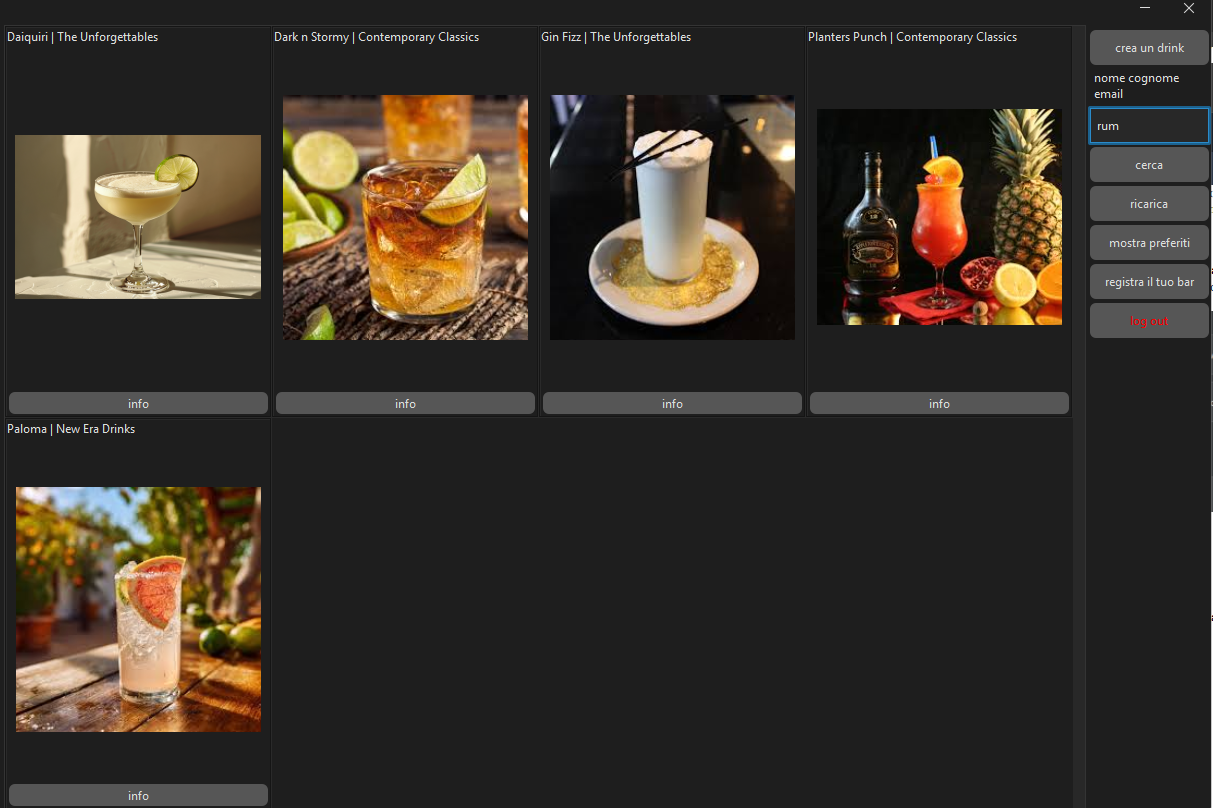
\includegraphics[width=1.0\linewidth]{images/applicazione/ricercaParoleChiave.png}
    \caption{schermata di visualizzazione dei risultati delle ricerche}
    \label{fig:keyWordSearch}
\end{figure}

\label{*1} Ovviamente, è possibile cercare anche per nome, descrizione e parole chiave.

\newpage
\subsubsection{Creazione drink e bar}
\begin{figure}[H]
    \centering
    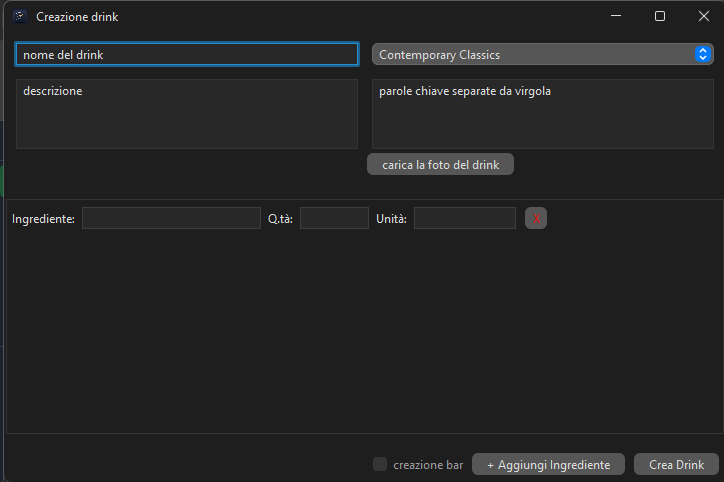
\includegraphics[width=0.9\linewidth]{images/applicazione/creazioneDrink.png}
    \caption{finestra di creazione drink}
    \label{fig:drinkCreation}
\end{figure}
\begin{figure}[H]
    \centering
    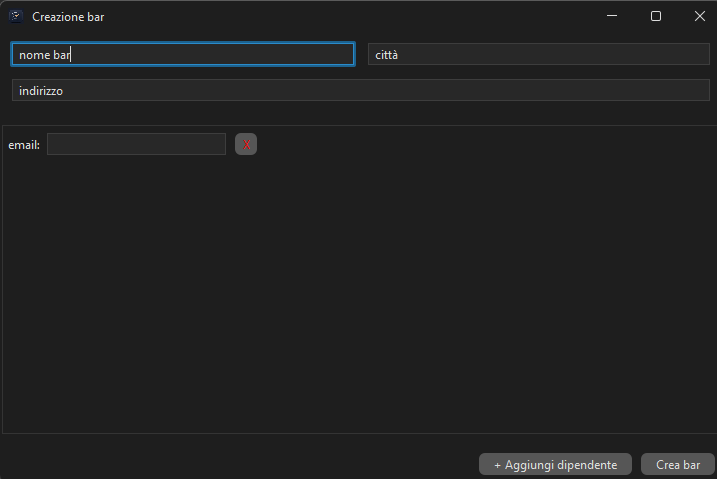
\includegraphics[width=0.9\linewidth]{images/applicazione/creazioneBar.png}
    \caption{finestra di creazione bar}
    \label{fig:barCreation}
\end{figure}


\subsubsection{Visualizzazione drink}

\begin{figure}[H]
    \centering
    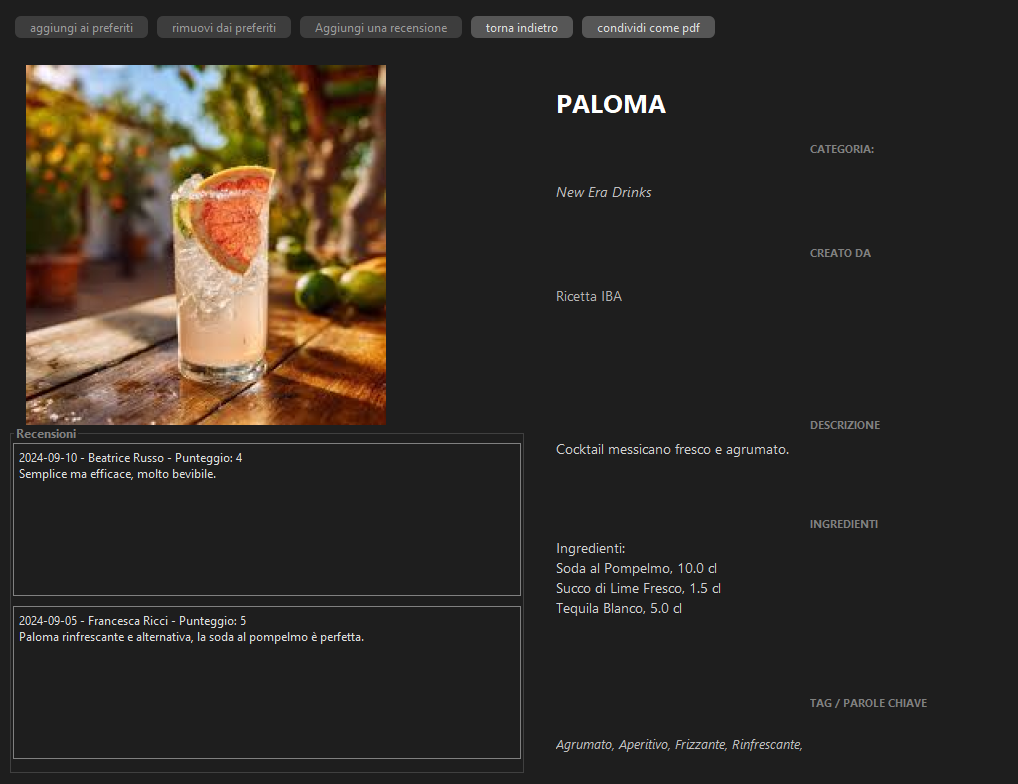
\includegraphics[width=0.8\linewidth]{images/applicazione/guestDrink.png}
    \caption{schermata di visualizzazione drink per gli ospiti}
    \label{fig:drinkInfoGuest}
\end{figure}
\begin{figure}[H]
    \centering
    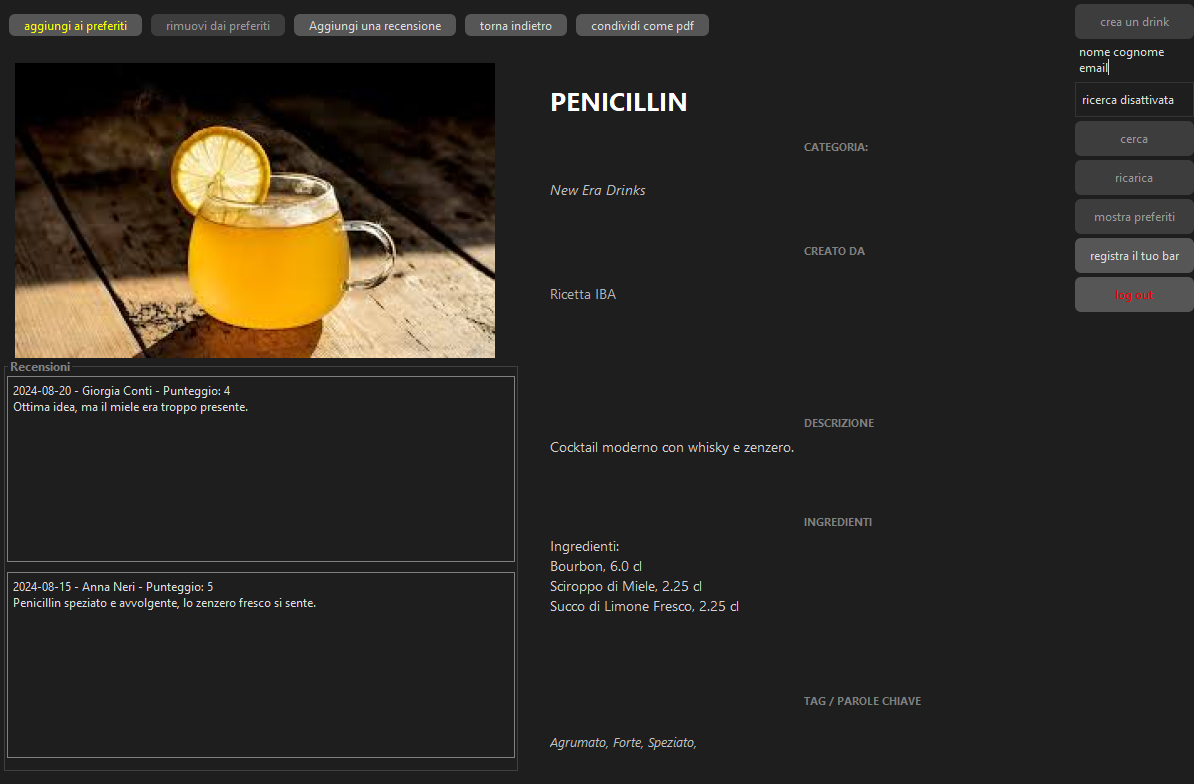
\includegraphics[width=0.8\linewidth]{images/applicazione/visualizzazioneDrink.png}
    \caption{schermata di visualizzazione drink per gli utenti registrati}
    \label{fig:drinkInfoUser}
\end{figure}

\subsubsection{Classifiche}
Le classifiche sono sempre visibili, nel pannello sinistro, come si vede in figura \ref{fig:leaderboards}
\begin{figure}[H]
    \centering
    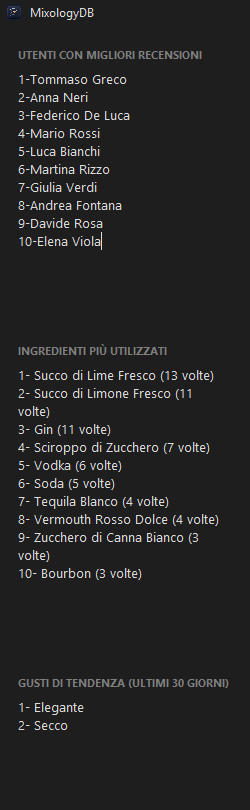
\includegraphics[width=0.35\linewidth]{images/applicazione/leaderBoards.png}
    \caption{Classifiche}
    \label{fig:leaderboards}
\end{figure}

\newpage
\subsubsection{Condivisione}
E' possibile condividere le ricette come file pdf (figura \ref{fig:share})

\begin{figure}[H]
    \centering
    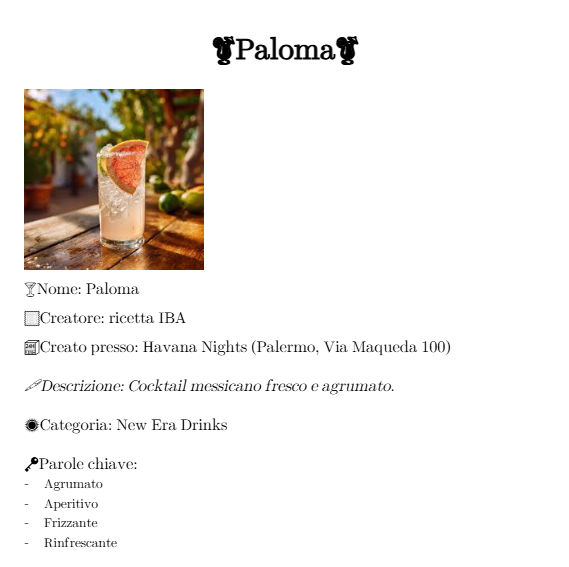
\includegraphics[width=1.0\linewidth]{images/share.png}
    \caption{file pdf esportato dall'applicazione}
    \label{fig:share}
\end{figure}

\newpage
\subsubsection{Funzioni riservate agli admin}
\begin{figure}[H]
    \centering
    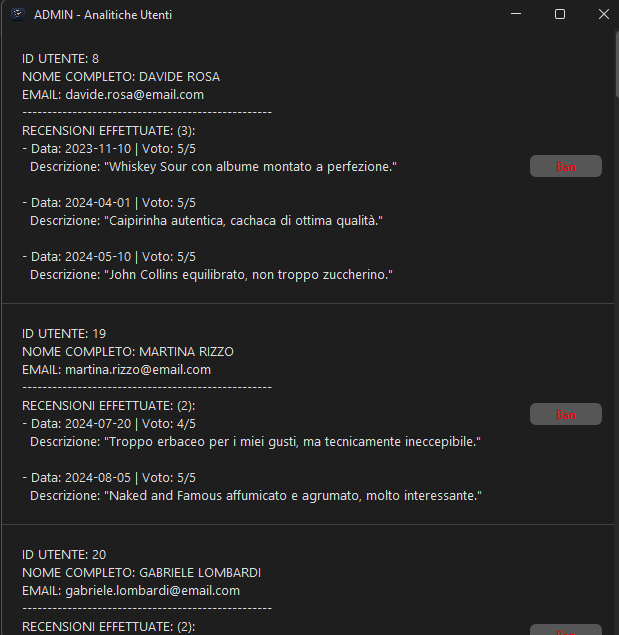
\includegraphics[width=0.6\linewidth]{images/applicazione/adminAnalitics.png}
    \caption{Visualizzazione dei dati analitici degli utenti}
    \label{fig:useranalitics}
\end{figure}
\begin{figure}[H]
    \centering
    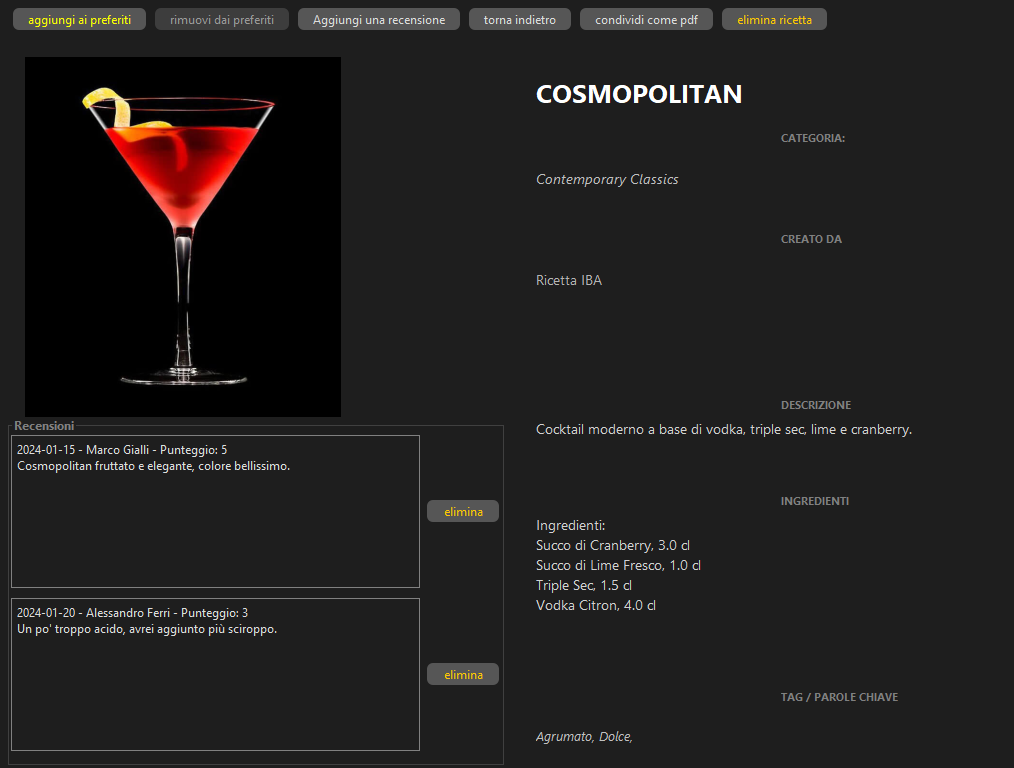
\includegraphics[width=0.6\linewidth]{images/applicazione/adminDrinkInfoPanel.png}
    \caption{schermata di visualizzazione drink con controlli admin}
    \label{fig:adminDrinkInfoPanel}
\end{figure}

\subsubsection{Link al repository}
\url{https://github.com/2menc/MixologyDB.git}
\end{document}
